\section{Analysis of the application from architectural point of view}
Modeling an information system implies a variety of activities, who have as primary descriptor the parallel handling of large information volumes. Earlier, in the requirements phase, it was built a conceptual model of the problem that identifies
what objects or entities are involved, what they look like (by defining their attributes), and how they relate
to one another. Now, it is the moment to describe the entire software structure, including all the interfaces, classes, interaction between users and system and more important - the interaction between system components. In order to characterize the inClass system, a collection of models were used:
\begin{itemize}
\item Use Case model. It is the representation of a user's interaction with the implemented system. Also it shows the different types of users and the various ways of interaction with the designed system.
\item Activity model. This type of models are aimed to display the overall flow of control in system, by modeling the computational and organizational processes (work-flows).
\item Sequence model. This is an interaction diagram, that shows how processes operate with one another and in what order. It is a collection of interactions arranged in time sequence.
\item Database model. It is a static structure diagram, which emphases which are the entities where the data are stored in the system and what type of relations exist between them. The same diagram contains all the attributes of each table and the connections between them (primary and foreign keys).
\item Deployment model. It shows what hardware and software components were used to setup the whole environment for designed system, \cite{diagrams}.
\end{itemize}
This is the chapter where the system is analyzed using the above enumerated types of diagrams, in order to get a more clear image about the system and its components interaction. Each diagram is designed to face the product from a concrete point of view, so that  it becomes straightforward how the system is built, works and which is the approach for future development.

\subsection{System requirements}
Speaking about the life cycle of a program, one of the basic levels to be taken into account is requirements specification towards the system. Covering this point helps the developer to determine which functionality the system is going to have for the future implementation. Usually, the requirements suffer changes during the development period, still it is vital to establish the basic ones since the beginning. As a matter of fact, versioning the system happens because testing the initial one rises some question marks, so the next product version comes with some revised requirements. One of the most important things that the discussed application should be able to do  is displaying the current academic timetables for a given type of user. Also, the veracity of the data should be taken into account, because the system needs maintenance with database records being in conformity with the current academic situation. 

Another moment of attention should be paid to the chosen framework and language for development of the system. Considering the environmental conditions, the best option would be creating a web application, assuming that the main target dispose of the necessary instruments for reaching the application: internet connection and suitable mobile phones. As a generalization, the system is expected to accomplish the following requirements:
\begin{itemize}
\item Allow different account types;
\item Create access boundaries for each type of user;
\item Create a database model that emphases the encountered real-life situation;
\item Permit creation of different types of entities, according to the database model;
\item Limit the scenario of account creation for teachers by delegating the task to the admin;
\item Allow student registration by invoking the specification of group of appurtenance
\item Permit editing current existing entities;
\item Display current timetable depending on individual profile;
\item Filter the courses by the corresponding labels for each user;
\item Display data according to current day of the week for both teacher and student;
\item Admit only one logged user per computer;
\item Visualize statistical information about user's activity for admins.
\end{itemize}

This are the first stage requirements established for the application, with possible future modification depending on the development directions. Future possible requirements can be linked by integration using the API of an already existing platform for enlarging the offered services. More specific details would imply courses visualization, together with the possibility of online access to regular tests or exams and grades assignment directly on the platform. Other directions for development could imply developing student's and teacher's profiles by creating additional features for them. 

At this moment the two types of users are limited only to data visualization. Creating additional options like daily reviews on the academic situation, some time management tools for course tasks organizing, interaction between the two types of users via announcements page would be some of the additional requirements for the second version of the system.

\subsection{Representation of the system via Use Case Diagrams}
The first diagram to be discussed presents the interaction of the administrator as actor in the system. For parallel visual observation, see \autoref{fig:University_Use_Case_Model}. All the Use Case diagrams have as prerequisite the fact that the user, no matter which type is it, must be logged in. If there is no account created, registration is required. The primal activity the administrator can perform with a fresh database is to create one of the global entities of the system, a new university. In order to create one, it is necessary to access the "Universities" option in the menu. After clicking on it, the page containing all the available universities will be rendered. At the moment, there are no universities in the system, that's why the list is empty, Besides the list of universities, there is an "Add University" button, which suggestively exhorts the user to click it. After clicking, the form for creating new universities will be rendered bellow. This particular form contains the Edit Box, where the name of the university should be typed in and the "Submit" button, for accomplishing the procedure. Basically, this is how the "Create a new University" use case can be described. 

\begin{figure}[H]
\centering
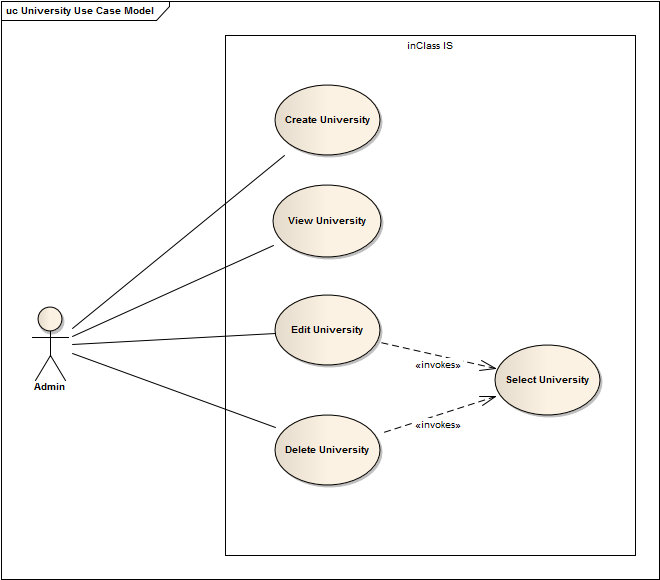
\includegraphics[width=14cm]{Chapter2/University_Use_Case_Model.png}
\caption{Use case diagram for Universities}
\label{fig:University_Use_Case_Model}
\end{figure}

After submitting the form, the university becomes immediately visible on the same page, in the mentioned list of universities. Besides the name of the university, on the right side, two buttons will become available for each new created entity. One of the buttons is for editing the current name of the selected university, the other one is for deletion. As a remark, should be mentioned that, as global entities in the database, deleting a university implies  all its content being recursively destroyed from the database. In order to edit the University, it is sufficient to click on the "Edit University" button and the edit form will be rendered. The form contains an Edit Box with current name in it and the "Submit" button. The name of the university becomes accessible for retyping and pressing "Submit" button will make the final changes in the database record.
\newpage

The next diagram shows the interaction between the same administrator with the system, by creating another type of entity. Assuming that at least one university already exists in the database, now it is possible to add components to it. For that, it is necessary to click on the University title for entering the general University page. It is quite similar with the index page of the universities, the only difference being the fact that here two types of components can be created: new faculties and new teachers. The \autoref{fig:Faculty_Use_Case_Model} shows the available use cases for dealing with faculties in the system. In order to create a new faculty, the admin has to enter the university page first. As no records are available at the moment, 2 empty lists will be displayed. The first one, visualizing faculties comes with an "Add faculty" button on the top. Clicking on the button will render the form for creating new faculties, which is similar with the one for creating universities. It also contains the Edit Box, where the name of the faculty should be typed in and the "Submit" button for data salvation. 

Adding new faculties will populate the list from the same page, so each of the new entries has the options foe editing and deletion available. For editing the faculty, it is necessary to click the "Edit Faculty" button and rewrite data from the rendered form. By clicking the "Delete Faculty" button, the record will be permanently erased from the database, and recursively will be removed all the child components from the respective faculty.  For visualization, there are two available options for this type of entities. One of them is via access from the "Universities" option in the menu, which ensures the user also with data manipulation (edit, delete), while accessing the "Faculties" option from the menu will give access only to visualize the existing data, ordered chronologically, depending on the last updates made to the faculties.

\begin{figure}[H]
\centering
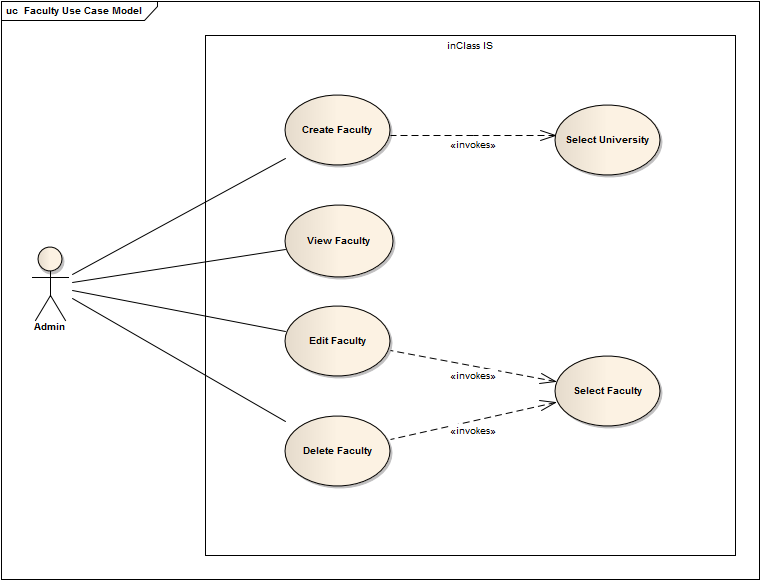
\includegraphics[width=14cm]{Chapter2/Faculty_Use_Case_Model.png}
\caption{Use case diagram for Faculties}
\label{fig:Faculty_Use_Case_Model}
\end{figure}
\newpage

Another illustration of a use case diagram is bringing the timetable model as one of the basic components of the system. It is created with the purpose of structuring the courses after a certain label. The Timetable is a child component of the Group. For every group, a single timetable can be created and it reflects the current ongoing semester. This means, that after each semester, when the timetables change, it is necessary to update the records by removing the current timetable and add a new one. The database is restricted to keeping one timetable per group, that's why creating a new timetable differs from the above described activities. In order to create a new timetable, a Group show page should be reached. Here, the standard "Add timetable" button is available. By clicking on it, the form for creating a new timetable is rendered. It contains a selection field, where only one option is available, the current semester for the group it belongs. By clicking the "Submit button", the record will be added in the database. This entities also have attached edit and delete buttons. The only difference is the editing process, that makes possible the partial update of the timetable's name by updating the name of the implicated group, in case that group suffered prior changes. Also, at this point, 2 more actors appear into the scenario for data visualization.More details will be discussed in the next paragraph. The \autoref{fig:Timetable_Use_Case_Model} presents the diagram discussed above:

\begin{figure}[H]
\centering
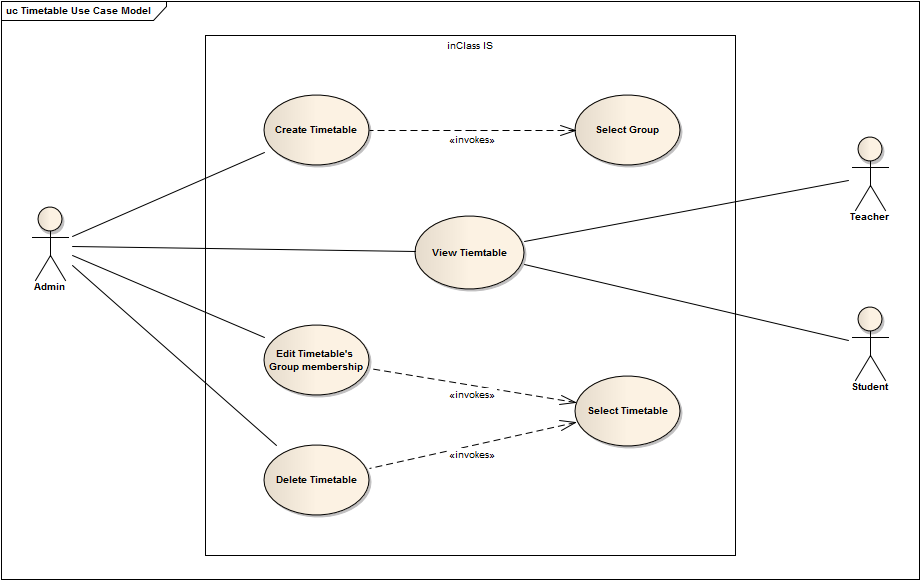
\includegraphics[width=14cm]{Chapter2/Timetable_Use_Case_Model.png}
\caption{Use case diagram for Timetables}
\label{fig:Timetable_Use_Case_Model}
\end{figure}

Reaching this point means that, in general lines, the system was completely analyzed via use case diagrams. The courses are the most low-level entities, which are basically the reason why the inClass application was developed. For parallel observation, see the \autoref{fig:Course_Use_Case_Model}. In order to be able to create a new course, a timetable show page should be involved. After entering it, the same template is used. An "Add Course" button is immediately available on the top of the page and by clicking it, the application redirects to a specific form for course creation. It contains several fields like course name, starting hour, teacher who is in charge for it, room where it takes place and day when it happens. A part of the fields are rendered as Edit Boxes and the admin is free to enter whatever data he/she wants and there are some selection fields, where the options are limited. After all the fields are completed, the "Submit" button saves the new record into the database. 

For every day of the week, a different table is generated. Also, the tables are ordered, starting with the first academic day of the week, Monday and finishing with the last one - Friday. Depending on the specified starting hour of the course, the records in the table are also sorted in ascending order. When the courses are created, three types of users in the system can visualize these data. The only difference is the type of accounts from which the courses are accessed and displayed. For editing the courses only the admin has permission, and the process flow is similar with the other discussed ones. For every course, edit and delete buttons are available and clicking those buttons have the same outcome as the ones previously addressed. 

\begin{figure}[H]
\centering
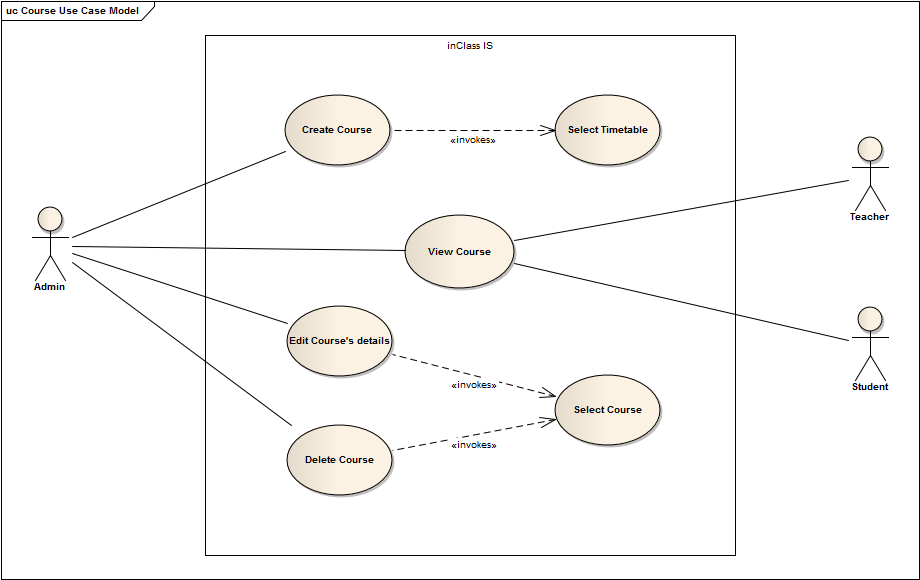
\includegraphics[width=14cm]{Chapter2/Course_Use_Case_Model.png}
\caption{Use case diagram for Courses}
\label{fig:Course_Use_Case_Model}
\end{figure}

\subsection{System Analysis using Activity Diagrams}
In the figure \autoref{fig:Create_Activity_Diagram_inClass}, illustrated bellow, is represented the flow of steps needed to be done in order to add a new Group record into the database. The user who has the rights to perform such operations in the system is the administrator. The first thing to be done in his/her case is to log-in. After reaching the application, the admin is ready to start the interaction with the system. To achieve the proposed goal, several primal entities need to be created or checked if exist. In this particular case, it is assumed the entities are missing and have to be created first. The process begins with accessing the "Universities" option from the menu. It is clear that the university that would contain such a group doesn't exist, so it must be added. 

The admin clicks on "Add University" button and starts introducing the name of the new recorded university. After submission, the new university becomes available as an element in the current list of universities in case the process was successfully accomplished. If not, an error message is displayed and the whole process starts from the beginning. Assuming the new record was created, clicking on the name of the university redirects the admin to the page where is shown the content of the current university. At the moment, the content is empty, so the admin proceeds to creating a new faculty. The process for adding a faculty is equivalent with the one of creating an university. After reaching the show page of the faculty, the admin is ready to create a new specialty. The process, one more time, coincides with the ones discussed above. At last, having a new specialty created, makes possible the event of adding the new group. Again, the admin presses on the "Add Group" button and enters the name of the group into the rendered form. If the submission of the new record is positive, the activity flow ends successfully. If something went wrong, an error message is displayed and the admin is one more time redirected to the specialty's show page. Here, the creation process starts all over.

Another interesting situation appears when the administrator tries to create a new timetable, but is not sure if the group for which the timetable should be created exists. In this case, he/she has two options. For time minimization purpose, the admin accesses, first of all, the "Groups" option in the menu. He/she navigates through the list of available groups and tries to find the one needed. If the group exists, the admin simply enters it and adds the new timetable by the same procedure discussed till now. If the group doesn't exist, a different path has to be covered. The admin chooses the option "Universities" from menu and starts navigating through faculties and specialties until reaches the list of all available groups. Here he/she adds a new one. Assuming the creation was successful, now it is possible to enter the group's show page. Here, the process of adding a new timetable is performed by accessing the form for creating new records of this type. If the process ends correctly, the new timetable becomes ready to be used. If not, the cyclic flow of steps are resumed. In the \autoref{fig:Add_Timetable_Activity_Diagram} the activity flow is represented graphically.

\begin{figure}[H]
\centering
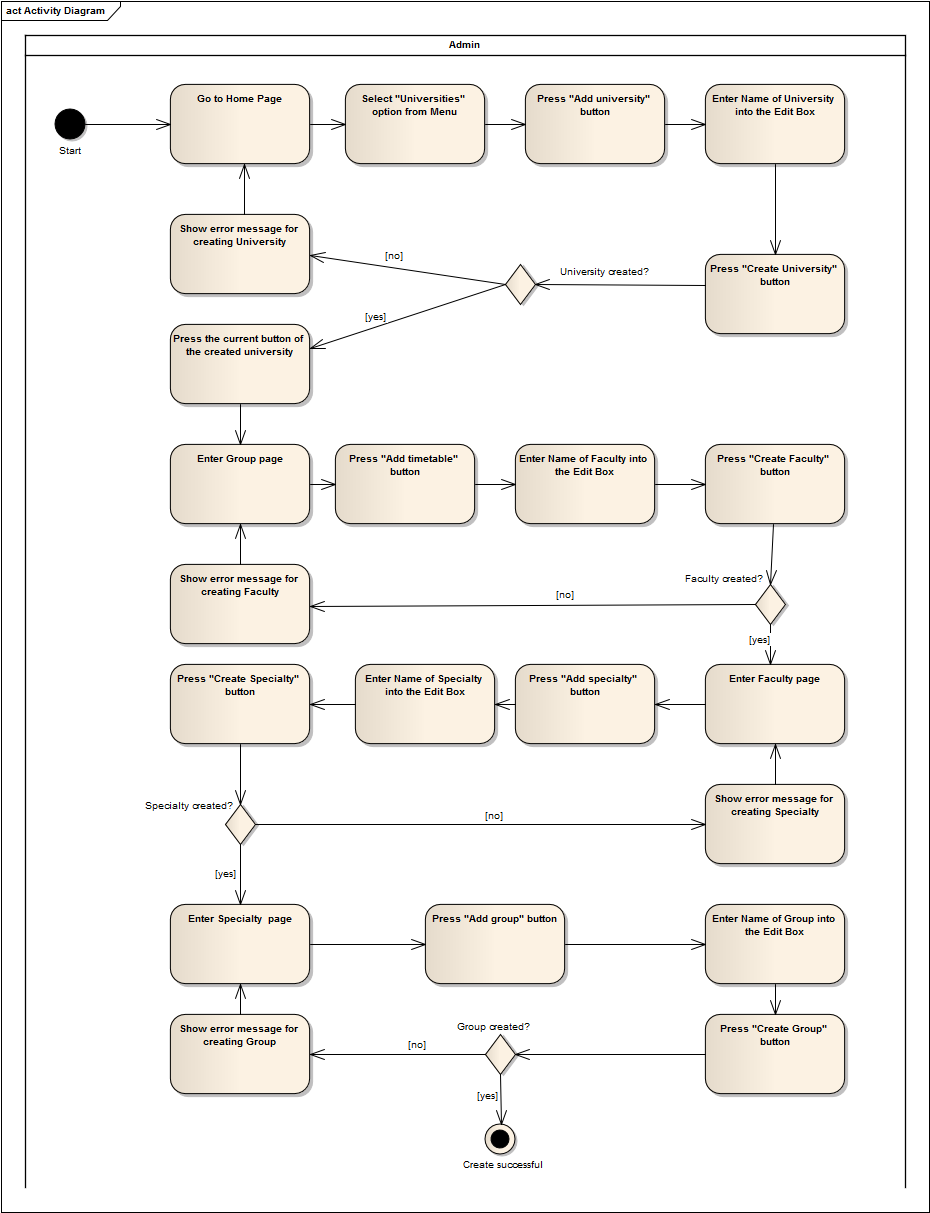
\includegraphics[width=18cm]{Chapter2/Create_Activity_Diagram_inClass.png}
\caption{Activity diagram for adding new Group}
\label{fig:Create_Activity_Diagram_inClass}
\end{figure}

\begin{figure}[H]
\centering
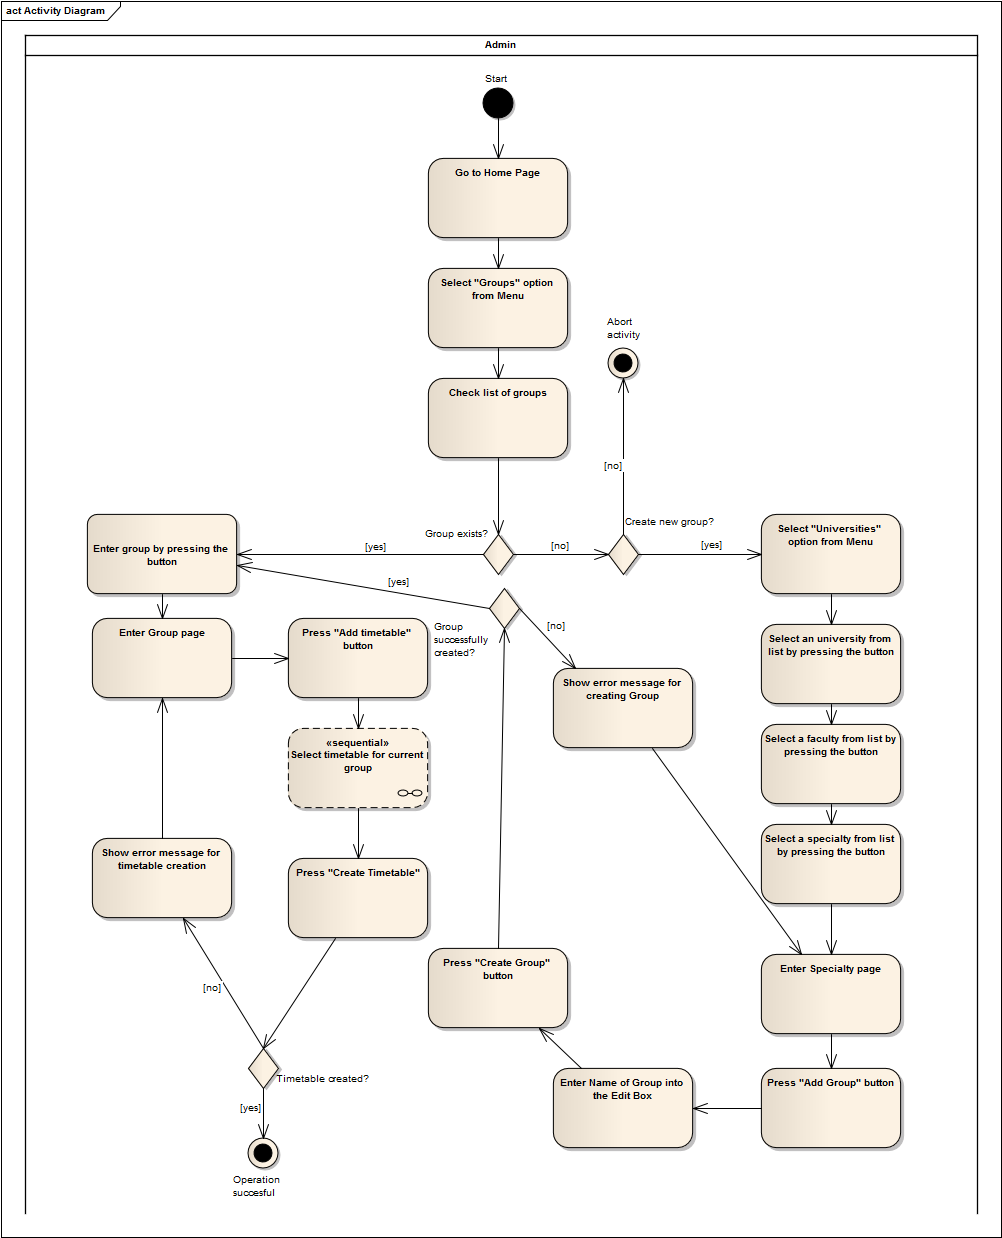
\includegraphics[width=18cm]{Chapter2/Add_Timetable_Activity_Diagram.png}
\caption{Activity diagram for adding new Timetable}
\label{fig:Add_Timetable_Activity_Diagram}
\end{figure}

\newpage
\subsection{Process interaction analysis using Sequence Diagram}
The sequence diagram is the one that shows how the smallest structural components, the processes, interact one with each other. As example, the action of editing an existing faculty was represented using this type of diagrams. The \autoref{fig:Sequence_Diagram} illustrates the UML description of the proposed activity, using the Enterprise Architect environment. 

So, in order to edit a faculty, it is necessary to access the application, go to the show page of a certain university and click on the "Edit faculty" button. What happens next is the loading of the corresponding view, passing as parameters the \texttt{university\_id} of the faculty and its own id. In Ruby, the forms are used just for representational and structural purpose, while the controllers are the entities that truly own the data. 

Obviously, the view now calls the \texttt{Faculties Controller} with the \texttt{edit} method. In the controller, first, a call to the \texttt{set\_university} method is made in order to find the parent university of the implicated faculty. The \texttt{find} function returns the \texttt{University} instance from the class, which has the specified \texttt{university\_id}. Now, in a local variable \texttt{faculty}, is stored the \texttt{Faculty} instance found in the \texttt{University} instance according to the \texttt{faculty\_id}. This local variable is then passed over to the view and the \texttt{edit} page is rendered, after the page is reloaded. Once the form is rendered, the updated name of the faculty is typed in the Edit Box. 

When the \texttt{Submit} button is clicked, the application passes the new \texttt{params} through the view and back to controller, where it calls the \texttt{update} method. This method finds the \texttt{Faculty} object by its id and stores it locally. After that, a check is preformed (by calling update method) for establishing if the new changes were applied having the \texttt{faculty\_params}. A boolean is returned as result which renders the university's home page if \texttt{true}, or renders the \texttt{edit} form again, if \texttt{false}.

\begin{figure}[H]
\centering
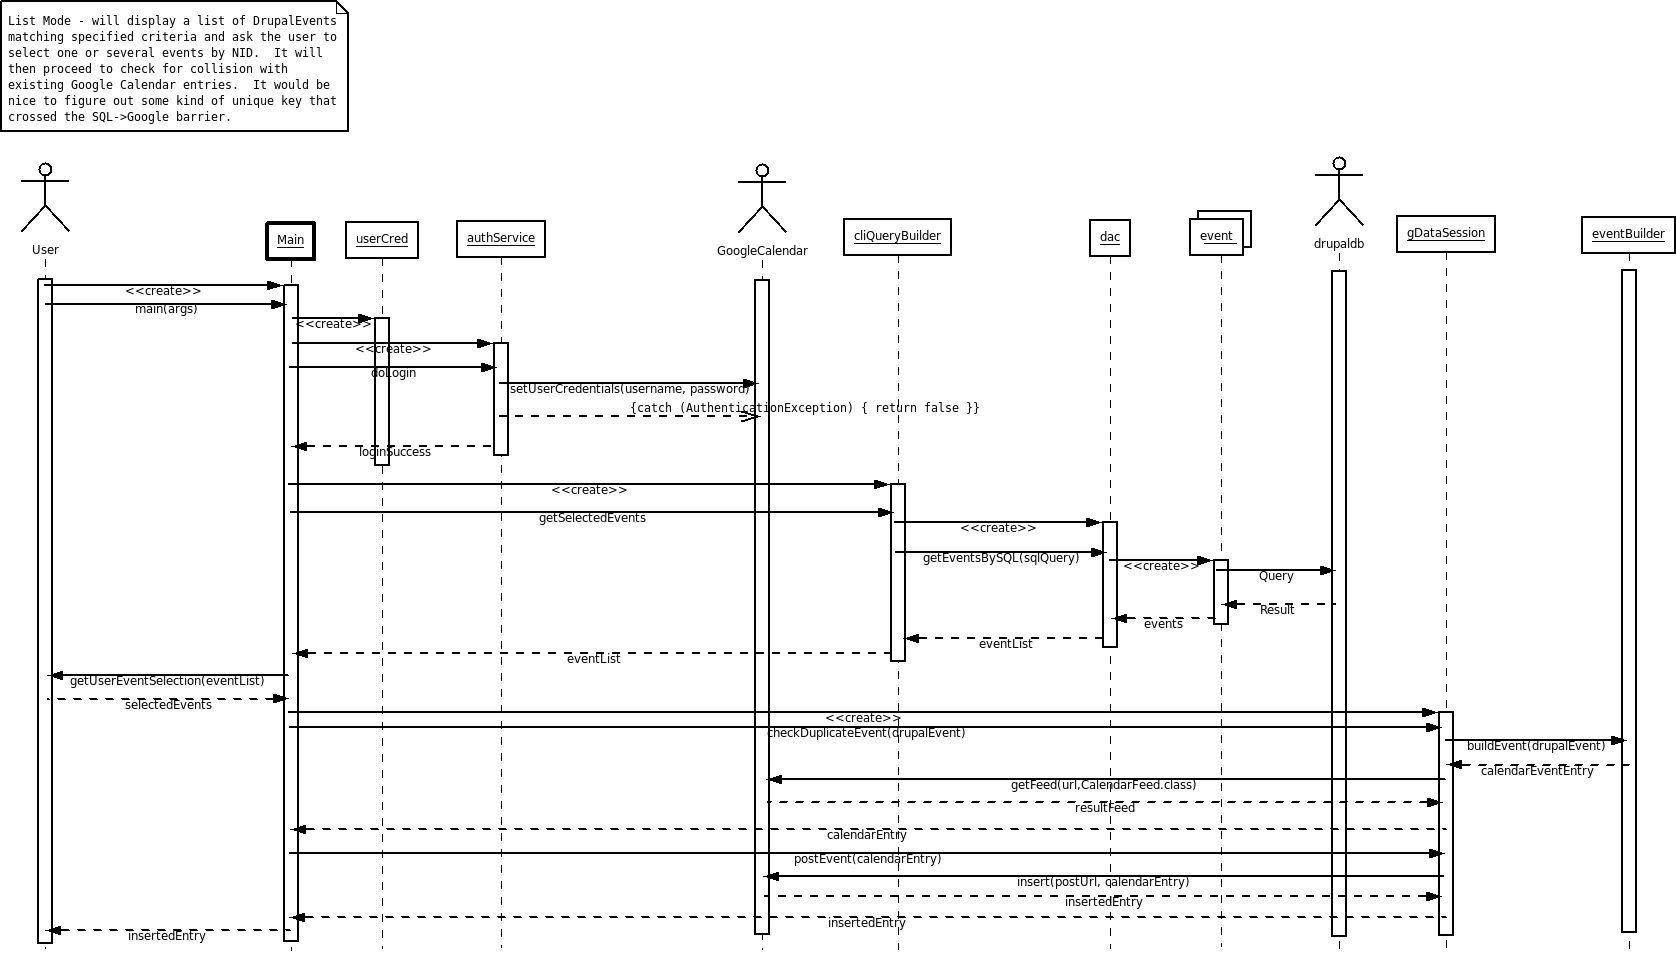
\includegraphics[width=18cm]{Chapter2/Sequence_Diagram.png}
\caption{Sequence Diagram for editing an existing Faculty}
\label{fig:Sequence_Diagram}
\end{figure}

\newpage
\subsection{The Database Model of the system}
Modeling how a system should store data is one of the primary steps to be done in the designing stage. Having a proper configuration of the database model guarantees an effective development of the required functionality. In \autoref{fig:database_diagram_inClass} 
is represented the database model which stands on the base of the system in discussion. Having defined the purpose of the application and the limits of functions it provides, it is mandatory to define the models that will store the data and the relationships between them. 

After analyzing the components of the system, it is clear that they have a tree structure. This means that the most general node is the University table. It contains several attributes like \texttt{title}, \texttt{creation date}, etc. and has as primary key the id it receives at creation. Following the Ruby convention, the \texttt{id} field is added automatically and is hidden in the schema. Still, it is there and developers know about that and this is the reason why all the tables have as primary keys these hidden fields. 

\begin{figure}[H]
\centering
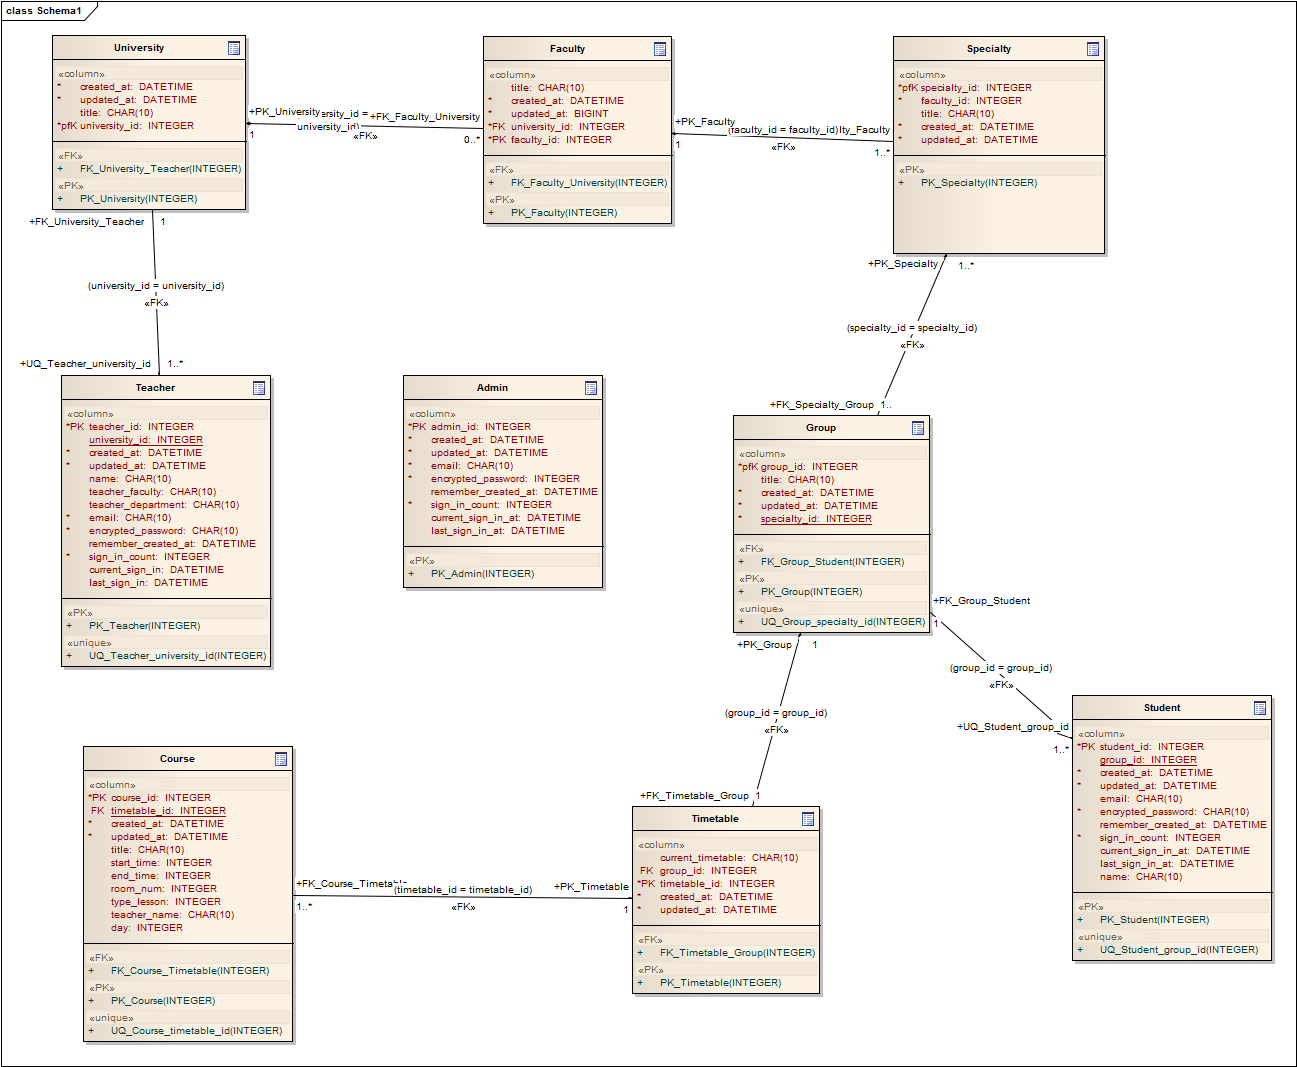
\includegraphics[width=18cm]{Chapter2/database_diagram_inClass.png}
\caption{Database model of the application}
\label{fig:database_diagram_inClass}
\end{figure}

\newpage
Now, applying the real - life model into the database structure, a university can have one or more faculties, meaning that the faculty has as foreign key the  \texttt{university\_id}, in order to create a relation between the two tables. The University is also linked via \texttt{university\_id} with the Teacher table, as the teachers are treated as entities belonging to a certain university. This fact was decided so, assuming that a teacher may teach courses to different faculties. Similarly, assuming that a faculty can have one or more specialties, a  \texttt{faculty\_id} attribute is specified in the Specialty table, as foreign key to the Faculty table. Now, a relation between a specialty and a group is established, assuming that a specialty has many groups and a group can belong just to one specialty. The  \texttt{specialty\_id} attribute is contained in the Group table as foreign key to Specialty table. 

From architectural point of view, it was established that the first version of the current application will contain only one timetable, reflecting the ongoing semester. That's why the Group can have only one Semester and the Semester can belong only to one Group. The  \texttt{group\_id} foreign key is contained in the Group table. Also a group should have one or more students, so another relation is established, the  \texttt{group\_id} being present in the Student table also as foreign key. Finally, every timetable should contain courses, so the Courses table is linked to Timetable via the  \texttt{timetable\_id} foreign key.

\subsection{Final stage of product development: Deployment Diagram}
At the deployment stage, it is assumed that the product is finished from development point of view and can be launched in production. Th \autoref{fig:Deployment_Model} materializes the components needed for release and the interaction between them that would guarantee a good functioning of the application as a complex system. 

The general deployment process consists of several interrelated activities with possible transitions between them.  It includes all the operations to prepare a system for assembly and transfer to the customer site. The resources required for deploying the current Ruby application involve 3 types of servers: an web server, an application server and a database server. The NginX web server was chosen for establishing an HTTPS connection with the PC via an web browser. Nginx uses an asynchronous event-driven approach to handling requests with modular event-driven architecture, providing more predictable performance under high loads. For the application server, Unicorn fits the best, assuming that is compatible with Ruby versions starting from 1.9.3 and is designed to serve fast clients on low-latency, high-bandwidth connections and take advantage of features in Unix/Unix-like kernels. Unicorn does not care if the application is thread-safe or not, workers all run within their own isolated address space and only serve one client at a time for maximum robustness. Combined with nginx and Ruby interpreter, any  binary upgrades are possible  without losing connections or dropping clients.

 The database server was chosen to be MySQL, which is the world's most popular open source relational database management system. It is an engine that effectively helps deliver high performance to scalable database applications, which is expected the current application to become, once it's released. In time, most probably, the application is going to operate with parallel database servers, to improve performance of  loading data, building indexes and evaluating queries.

\begin{figure}[H]
\centering
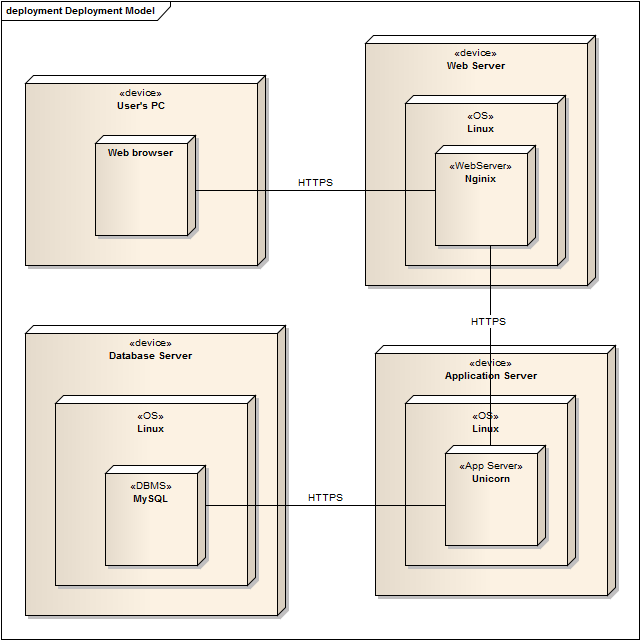
\includegraphics[width=14cm]{Chapter2/Deployment_Model.png}
\caption{Deployment model of the system}
\label{fig:Deployment_Model}
\end{figure}